\chapter{Neuen Workflow Erstellen}
    \begin{figure}[H]
        \centering
        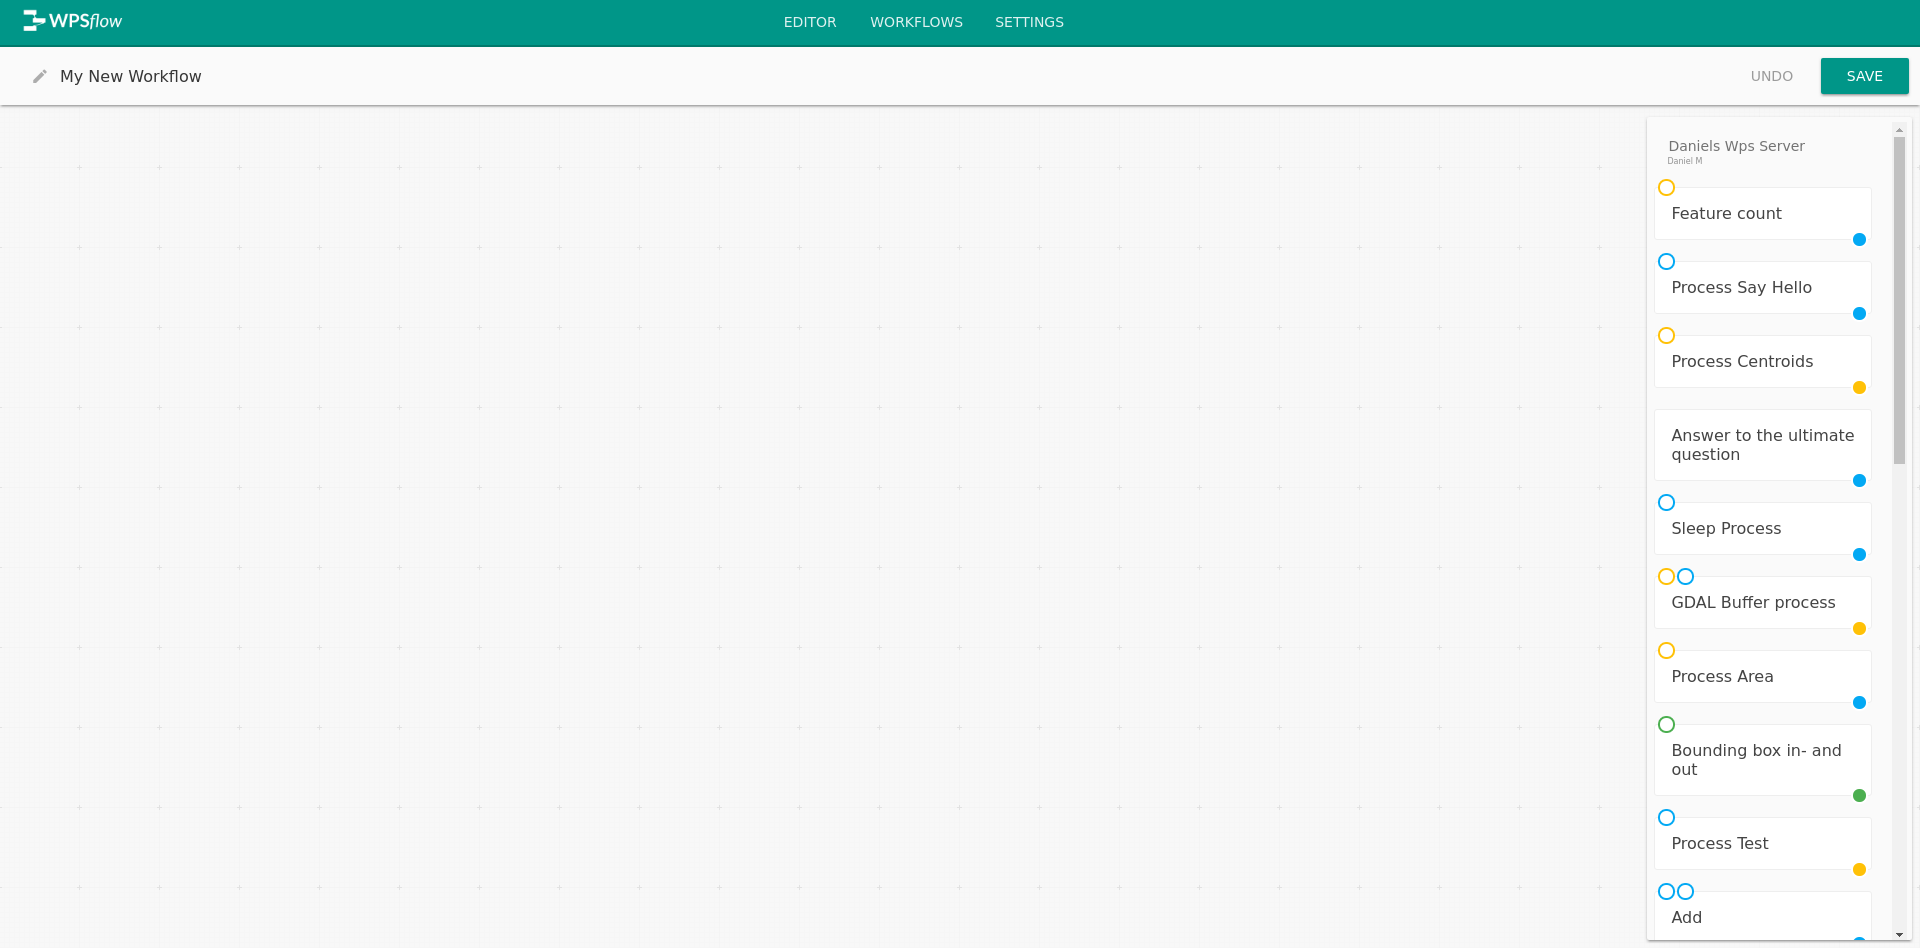
\includegraphics[width=15.5cm]{images/BaseEditor.png}
        \label{base_editor}
    \end{figure}
    Am Anfang ist der Basis Editor zu sehen. 
    \begin{figure}[H]
        \centering
        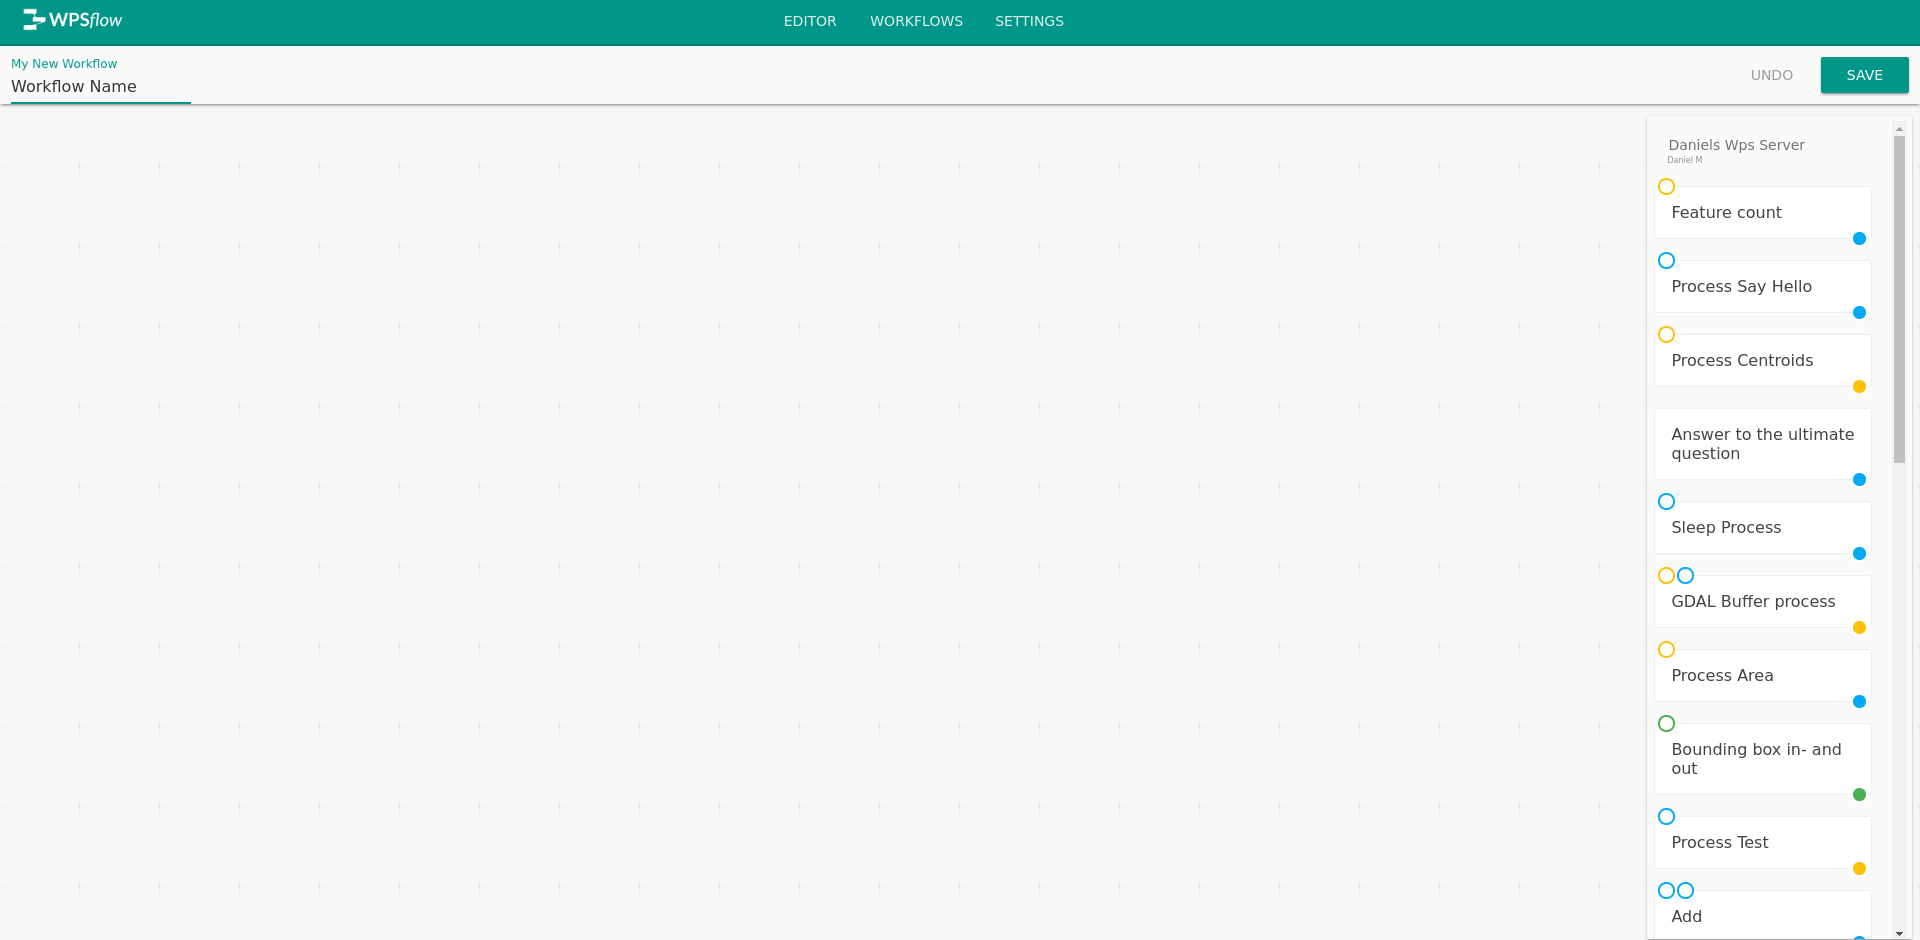
\includegraphics[width=15.5cm]{images/New Workflow.png}
        \label{new_workflow}
    \end{figure}
    \noindent Um einen neuen Workflow zu erstellen muss man zuerst einen neuen Namen eingeben. Dies kann man aber auch noch nachträglich machen. Dann ist speichern zu drücken um den neuen Workflow anzulegen. 
    
\chapter{Workflow Bearbeiten}
    \begin{figure}[H]
        \centering
        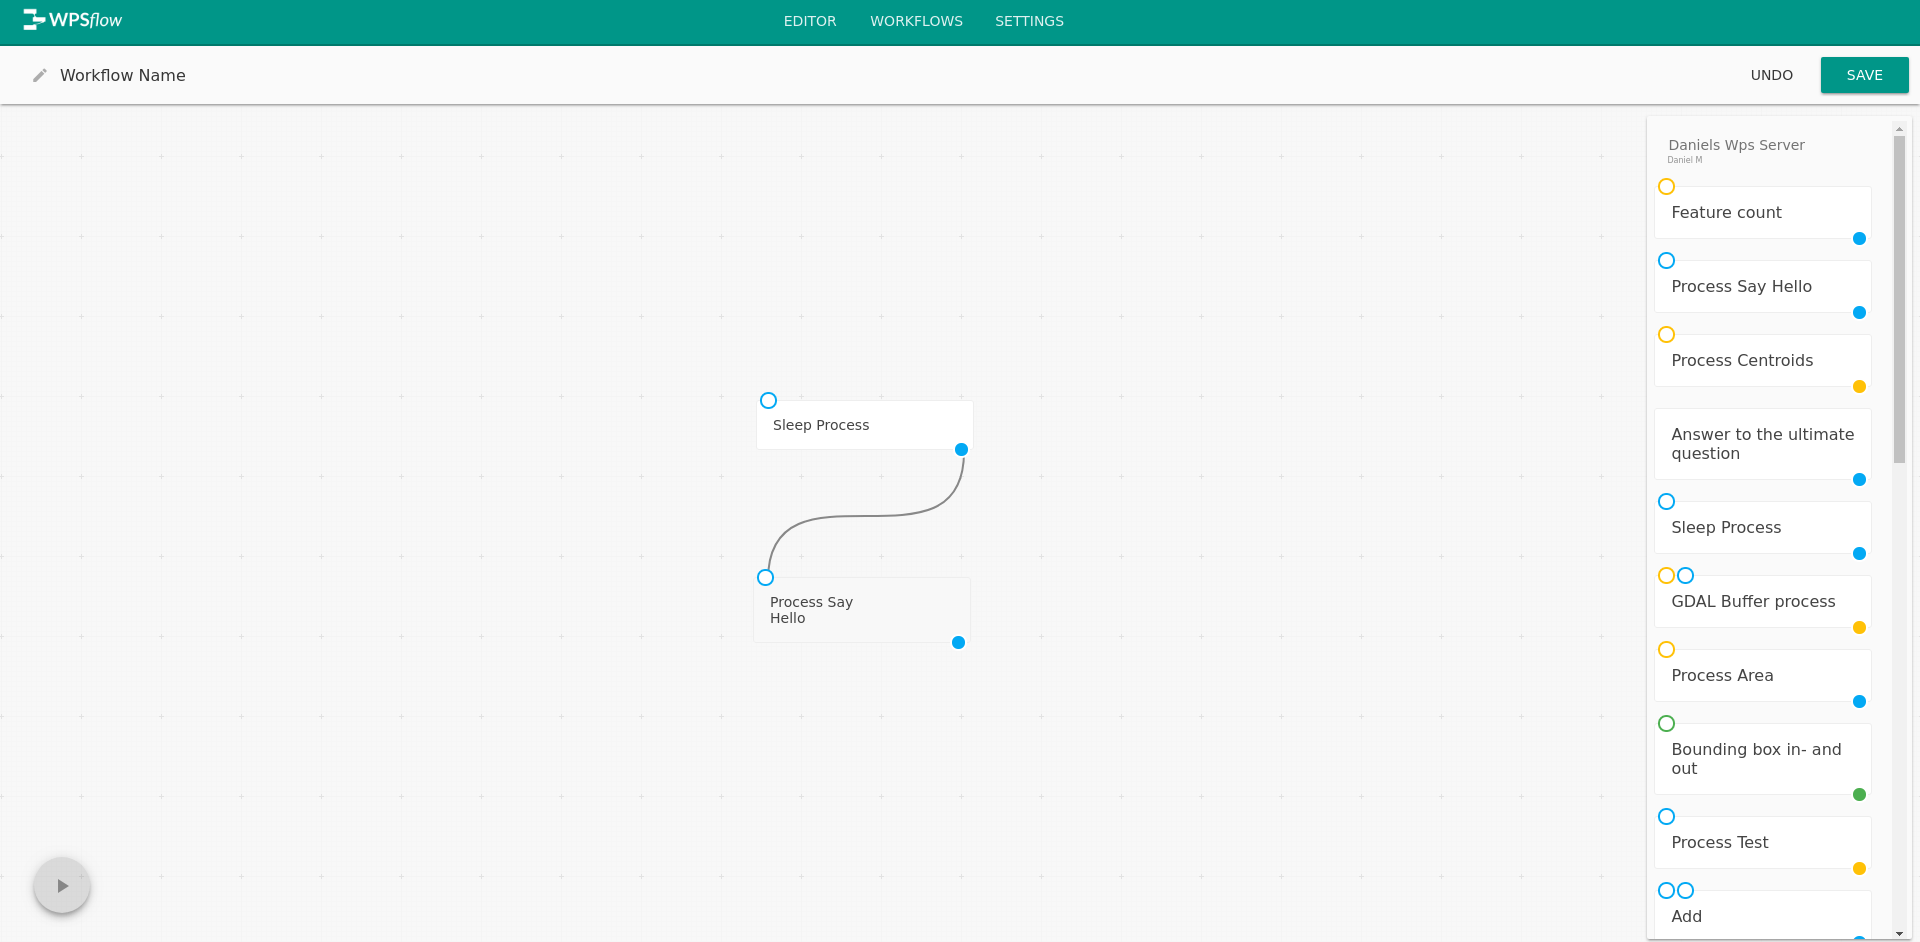
\includegraphics[width=15.5cm]{images/Create Workflow.png}
        \label{create_workflow}
    \end{figure}
    Anschließend kann man per Drag-n-Drop Tasks in den Workflow ziehen und die In- \& Outputs der Tasks miteinander verbinden. Änderungen kann man bequem mit dem speichern Knopf speichern. 
    \begin{figure}[H]
        \centering
        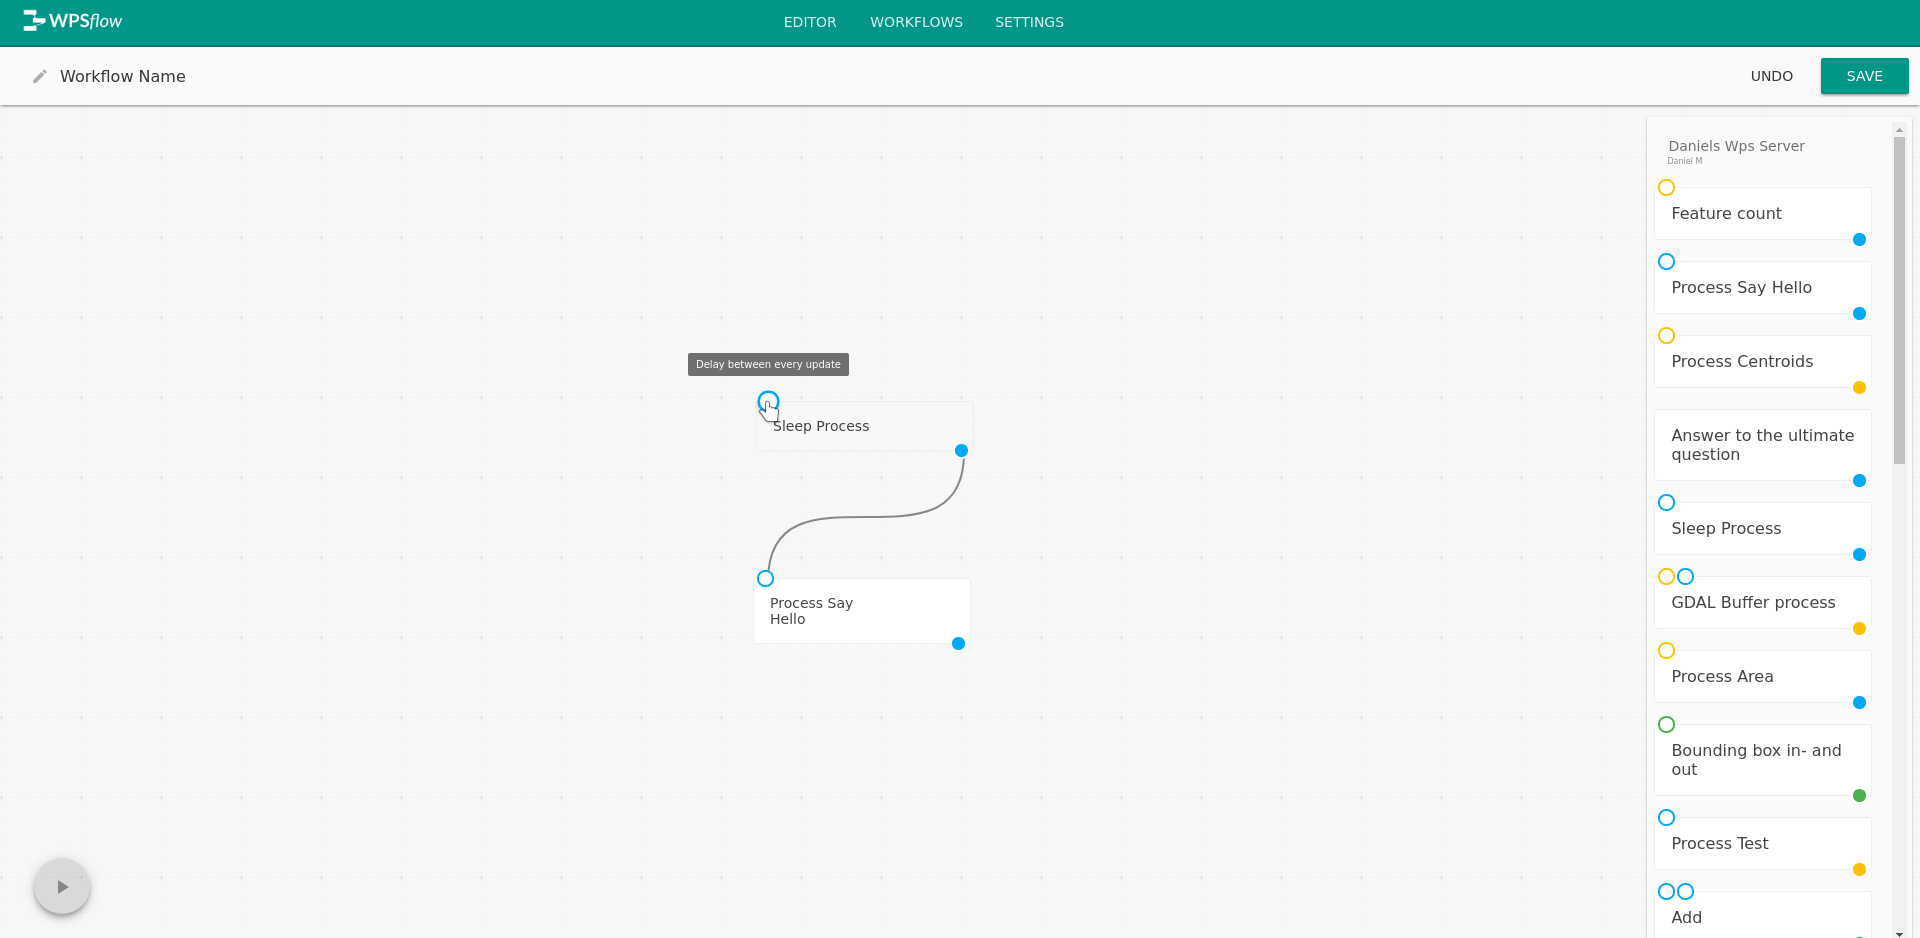
\includegraphics[width=15.5cm]{images/Add Input 1.png}
        \label{add_input_1}
    \end{figure}
    \noindent Um den Input eines Tasks manuell zu bestimmen ist einfach auf den Einganspunkt des Tasks zu klicken.
    \begin{figure}[H]
        \centering
        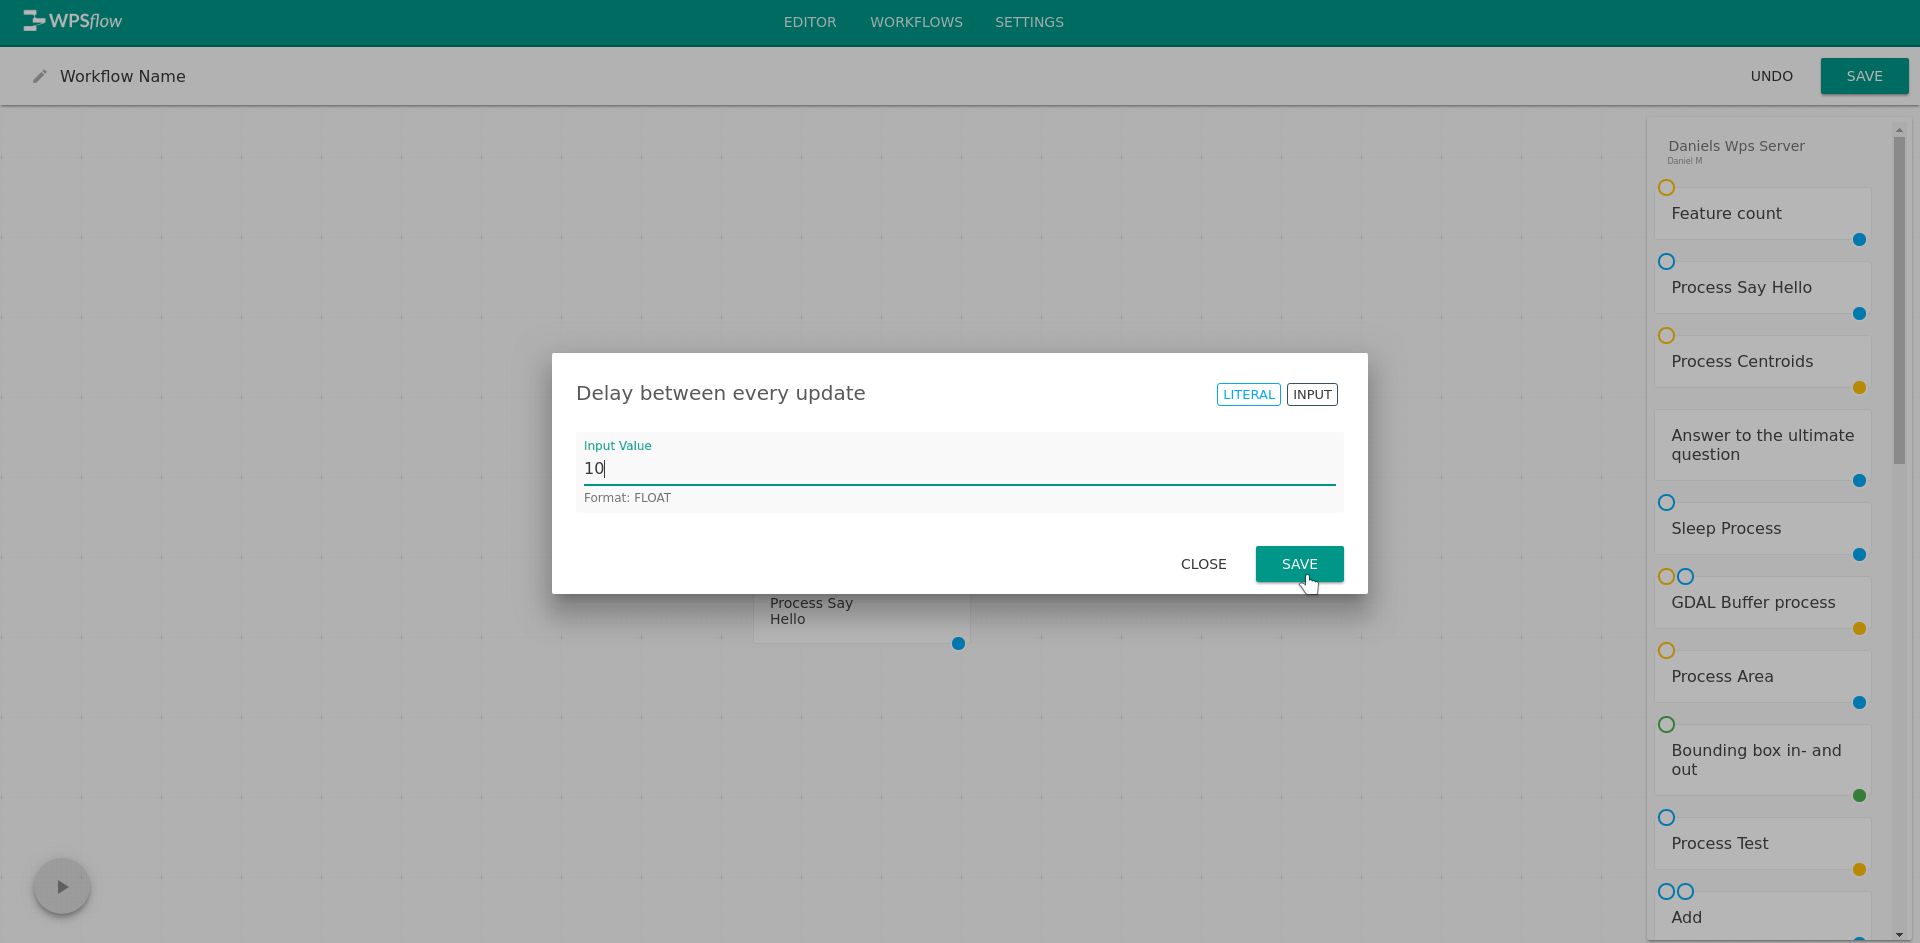
\includegraphics[width=15.5cm]{images/Add Input 2.png}
        \label{add_input_2}
    \end{figure}
    \noindent Hier öffnet sich dann ein Fenster, in das man die Daten eingeben kann, welche der Task verarbeiten sollen. Dieses Fenster ist mit dem speichern Knopf zu bestätigen. 
\chapter{Workflow Ausführen}
    \begin{figure}[H]
        \centering
        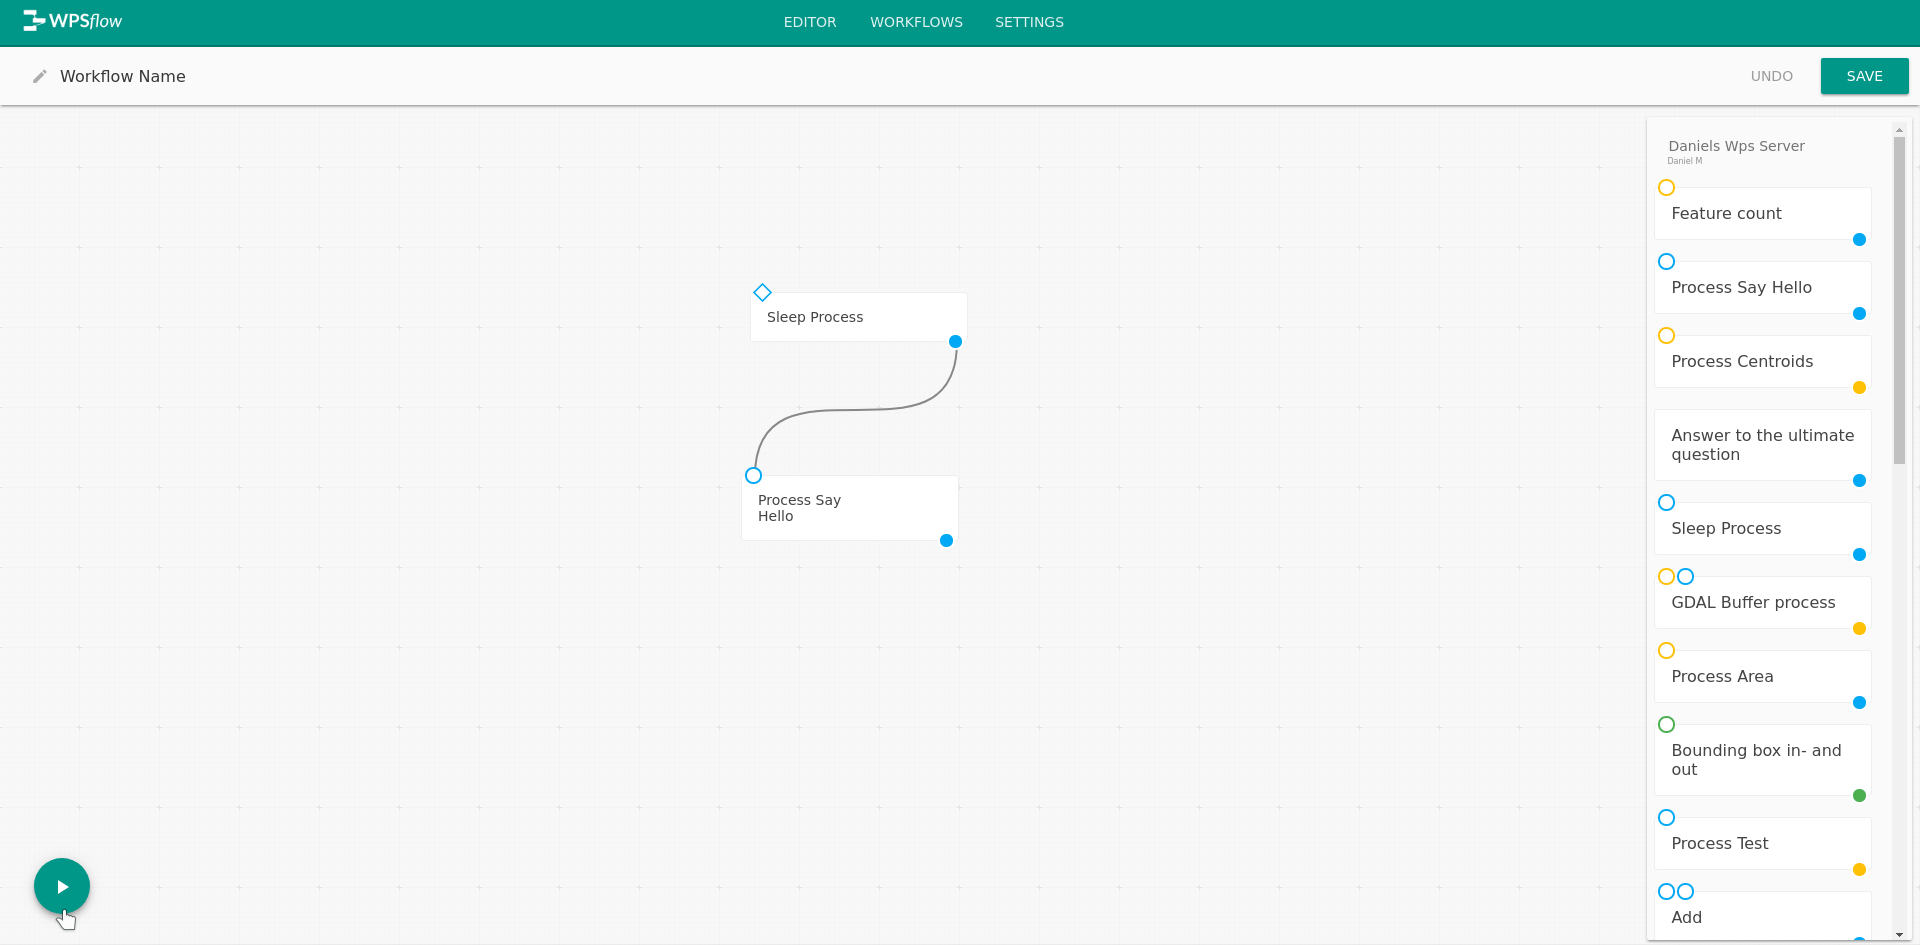
\includegraphics[width=15.5cm]{images/Start Workflow.png}
        \label{start_workflow}
    \end{figure}
    Jetzt wo der Workflow vollständig ist und eine korrekte Syntax aufweist, ist der ausführen Knopf unten links grün geworden. Drückt man diesen Knopf, kann man den Workflow nicht mehr bearbeiten, und er wird ausgeführt. 
    \begin{figure}[H]
        \centering
        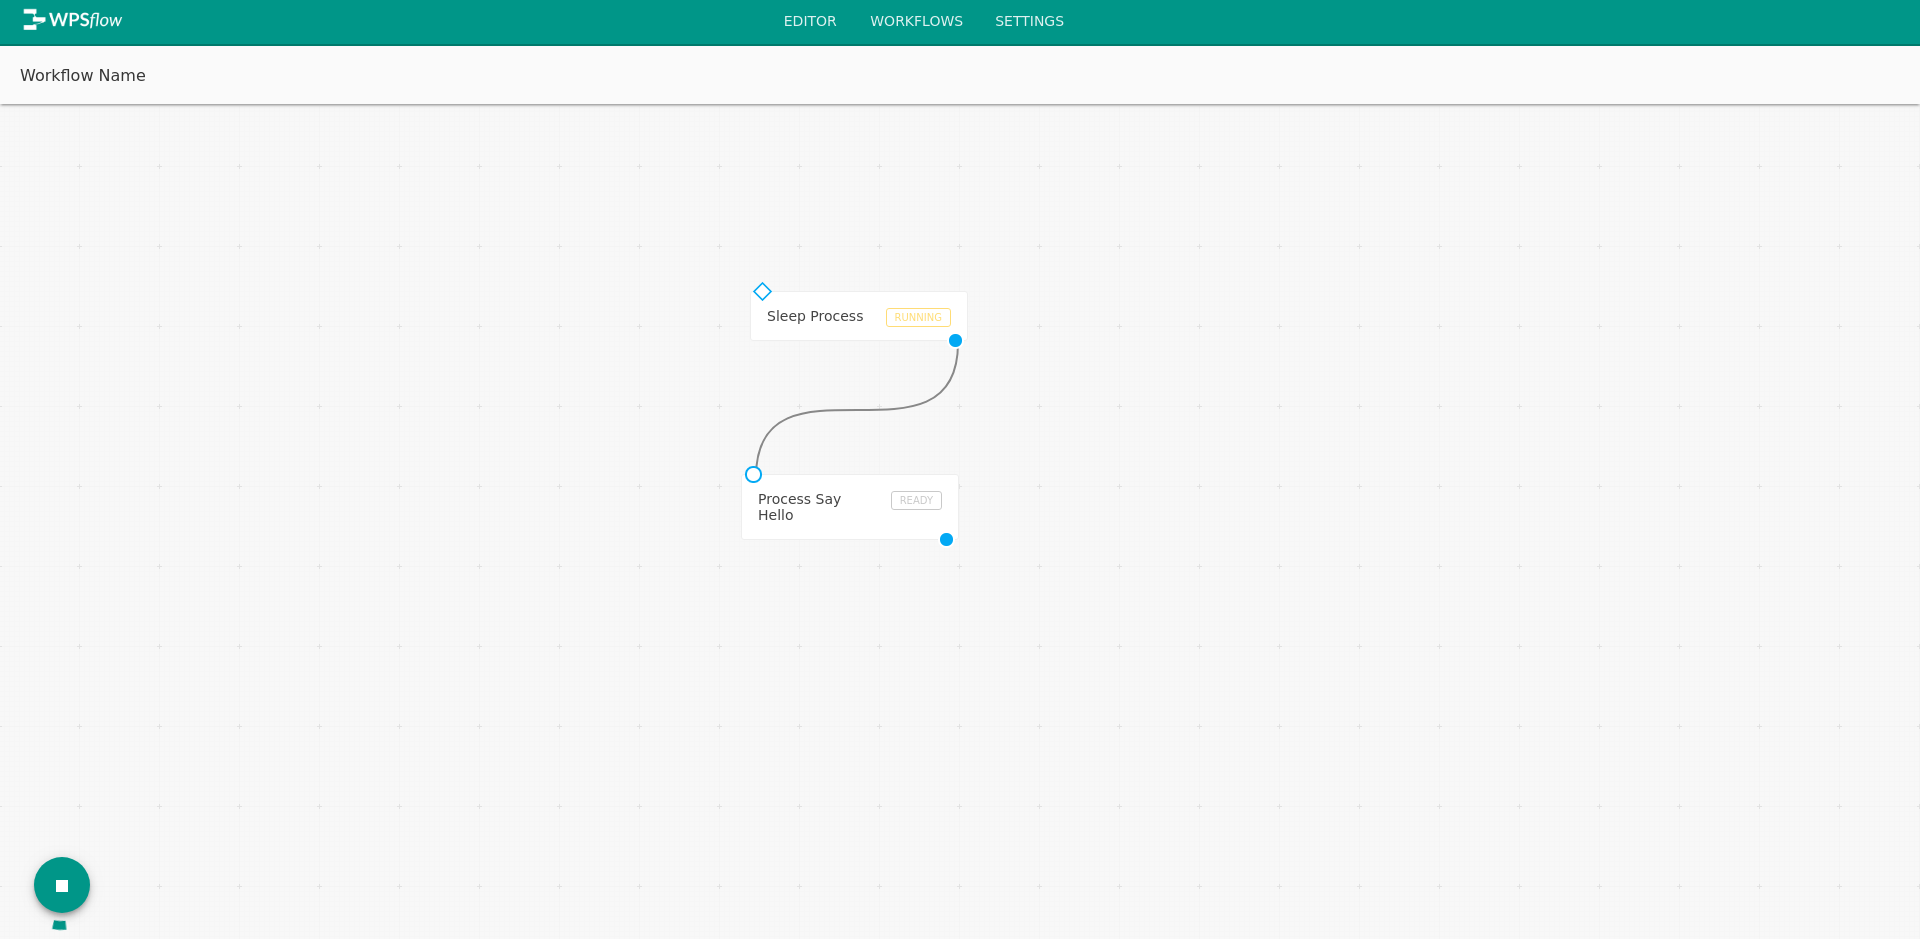
\includegraphics[width=15.5cm]{images/Running Workflow.png}
        \label{running_workflow}
    \end{figure}
    \noindent Ist die Ausführung des Workflows fertig, so kann man mit dem Knopf oben rechts, die Ergebnisse des Workflows anschauen. 
    \begin{figure}[H]
        \centering
        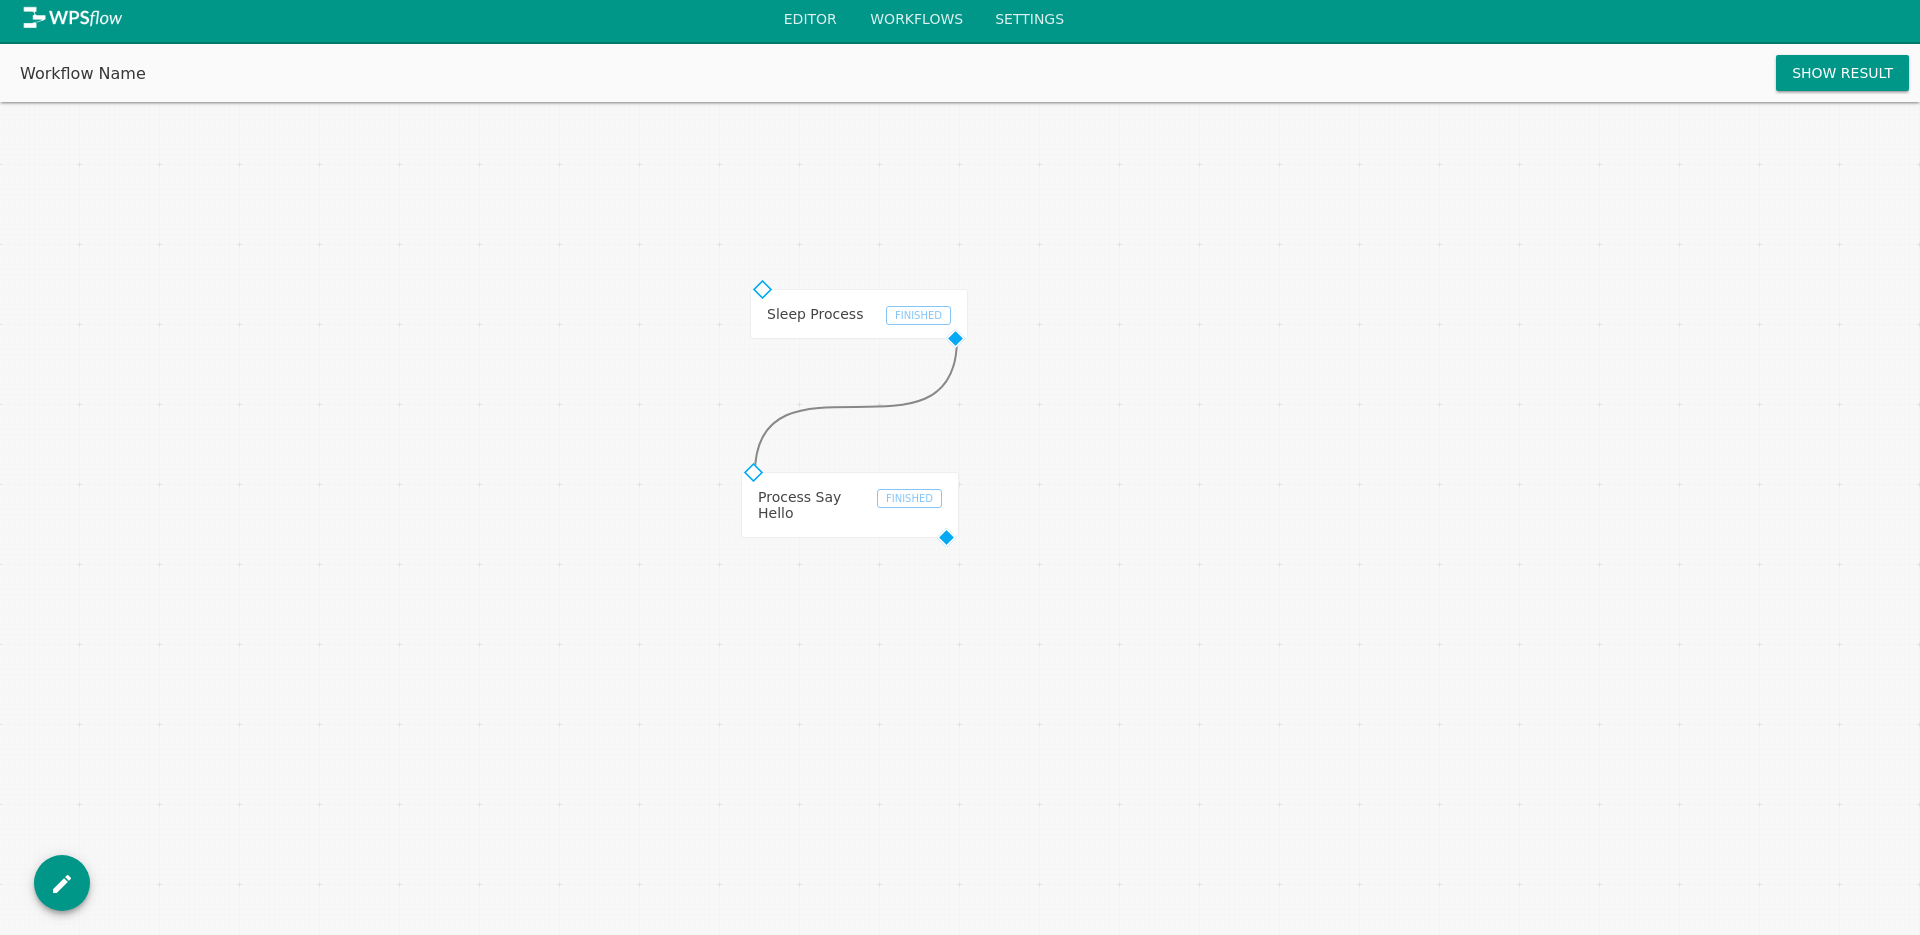
\includegraphics[width=15.5cm]{images/Finished Workflow.png}
        \label{finished_workflow}
    \end{figure}
    \noindent Dieses Fenster, mit den Workflow Ergebnissen, kann man mit wieder schließen, um auf der vorherigen Seite zu landen. Mit den Knopf unten links, kommt man wieder in den Bearbeitungsmodus, falls man etwas an dem Workflow anpassen möchte. 
    \begin{figure}[H]
        \centering
        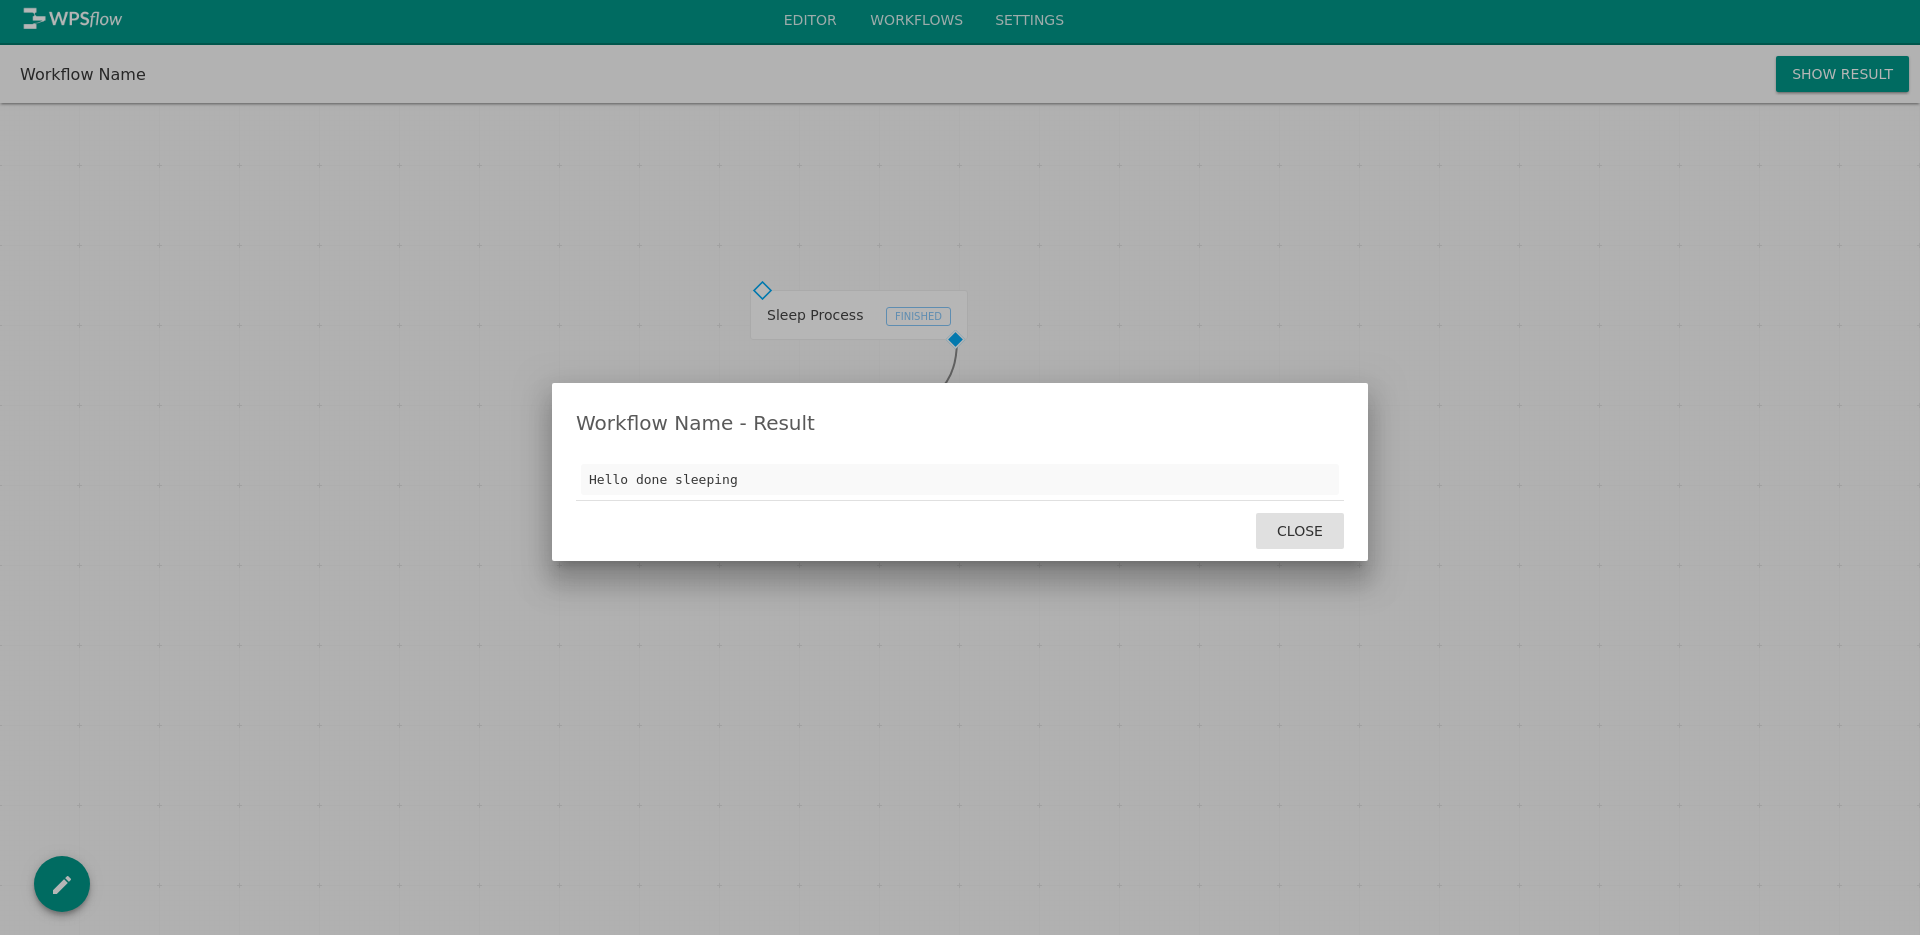
\includegraphics[width=15.5cm]{images/Workflow Result.png}
        \label{workflow_result}
    \end{figure}
    
\chapter{Workflow Übersicht}
    \begin{figure}[H]
        \centering
        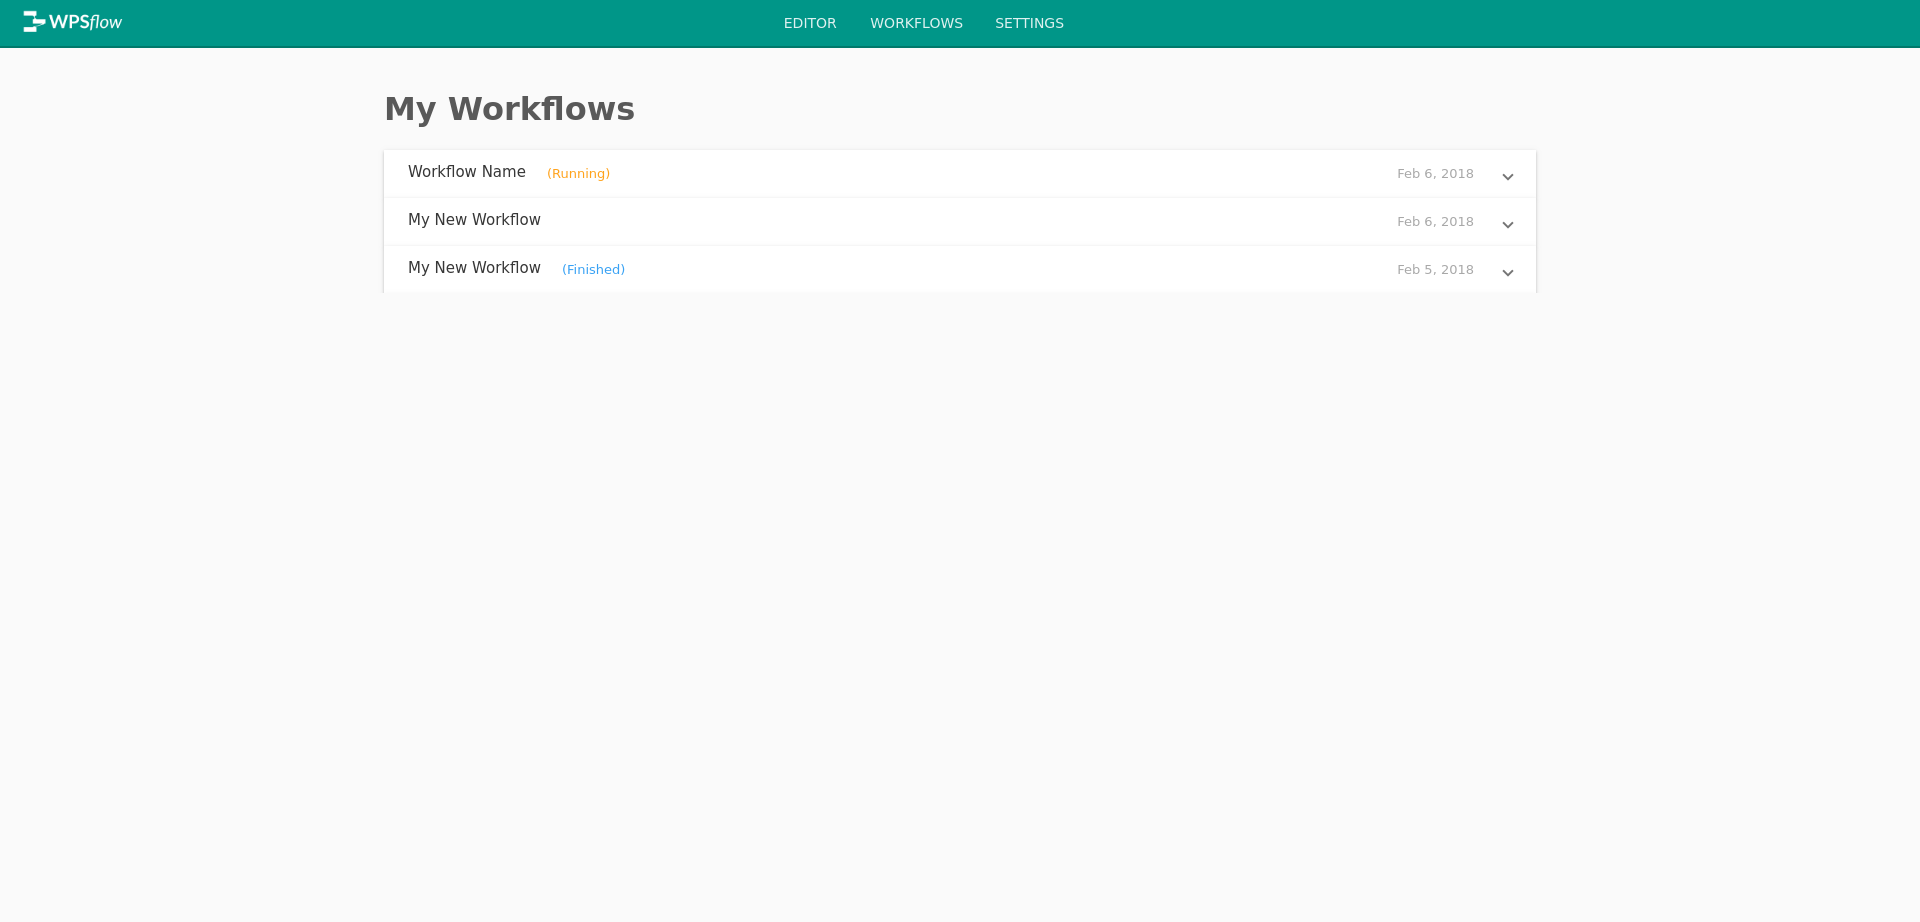
\includegraphics[width=15.5cm]{images/Workflow Overview.png}
        \label{workflow_overview}
    \end{figure}
    Drückt man auf den Knopf Workflow oben in der Mitte, landet man in der Übersichtanzeige seiner Workflows. Hier kann man sehen welche Workflows man angelegt hat bzw. die Ausführungsstatus der Workflows sehen. Wenn man einen Workflow anklickt, kann man diesen grob betrachten und diesen auch wieder bearbeiten, wenn man auf den bearbeiten Knopf drückt. 
    \begin{figure}[H]
        \centering
        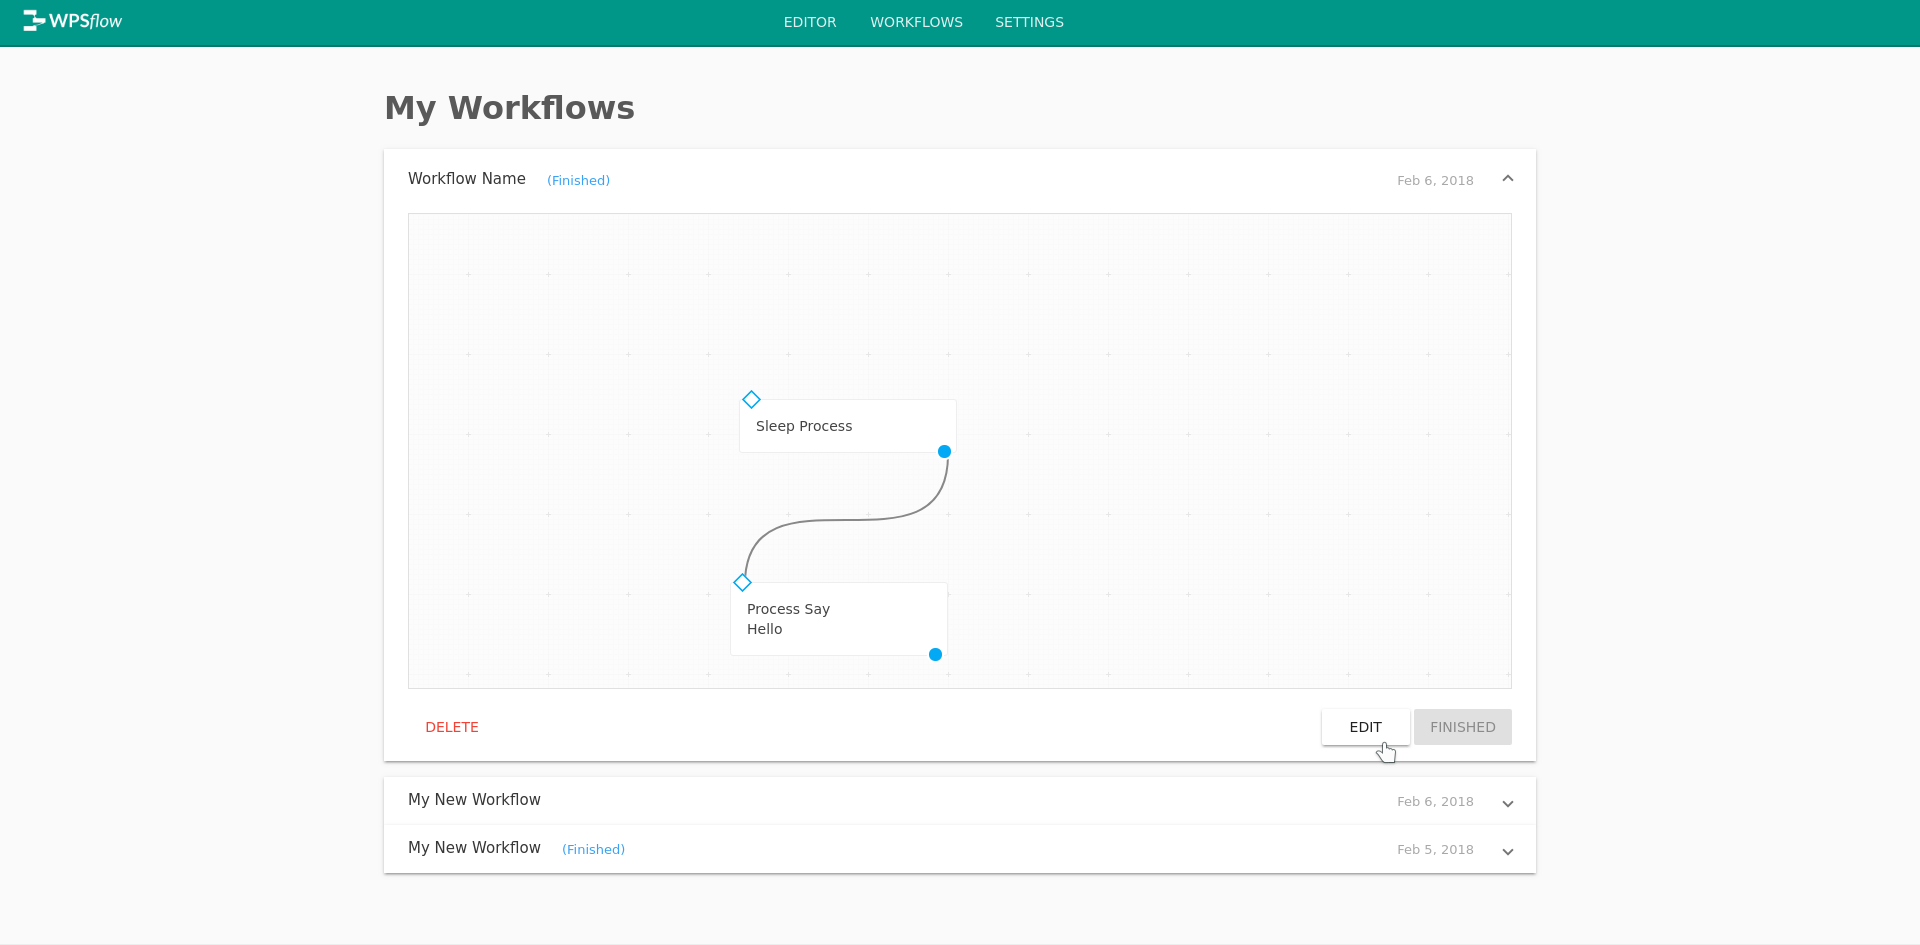
\includegraphics[width=15.5cm]{images/Choose Workflow.png}
        \label{choose_workflow}
    \end{figure}
    
\chapter{Einstellungen}
    \begin{figure}[H]
        \centering
        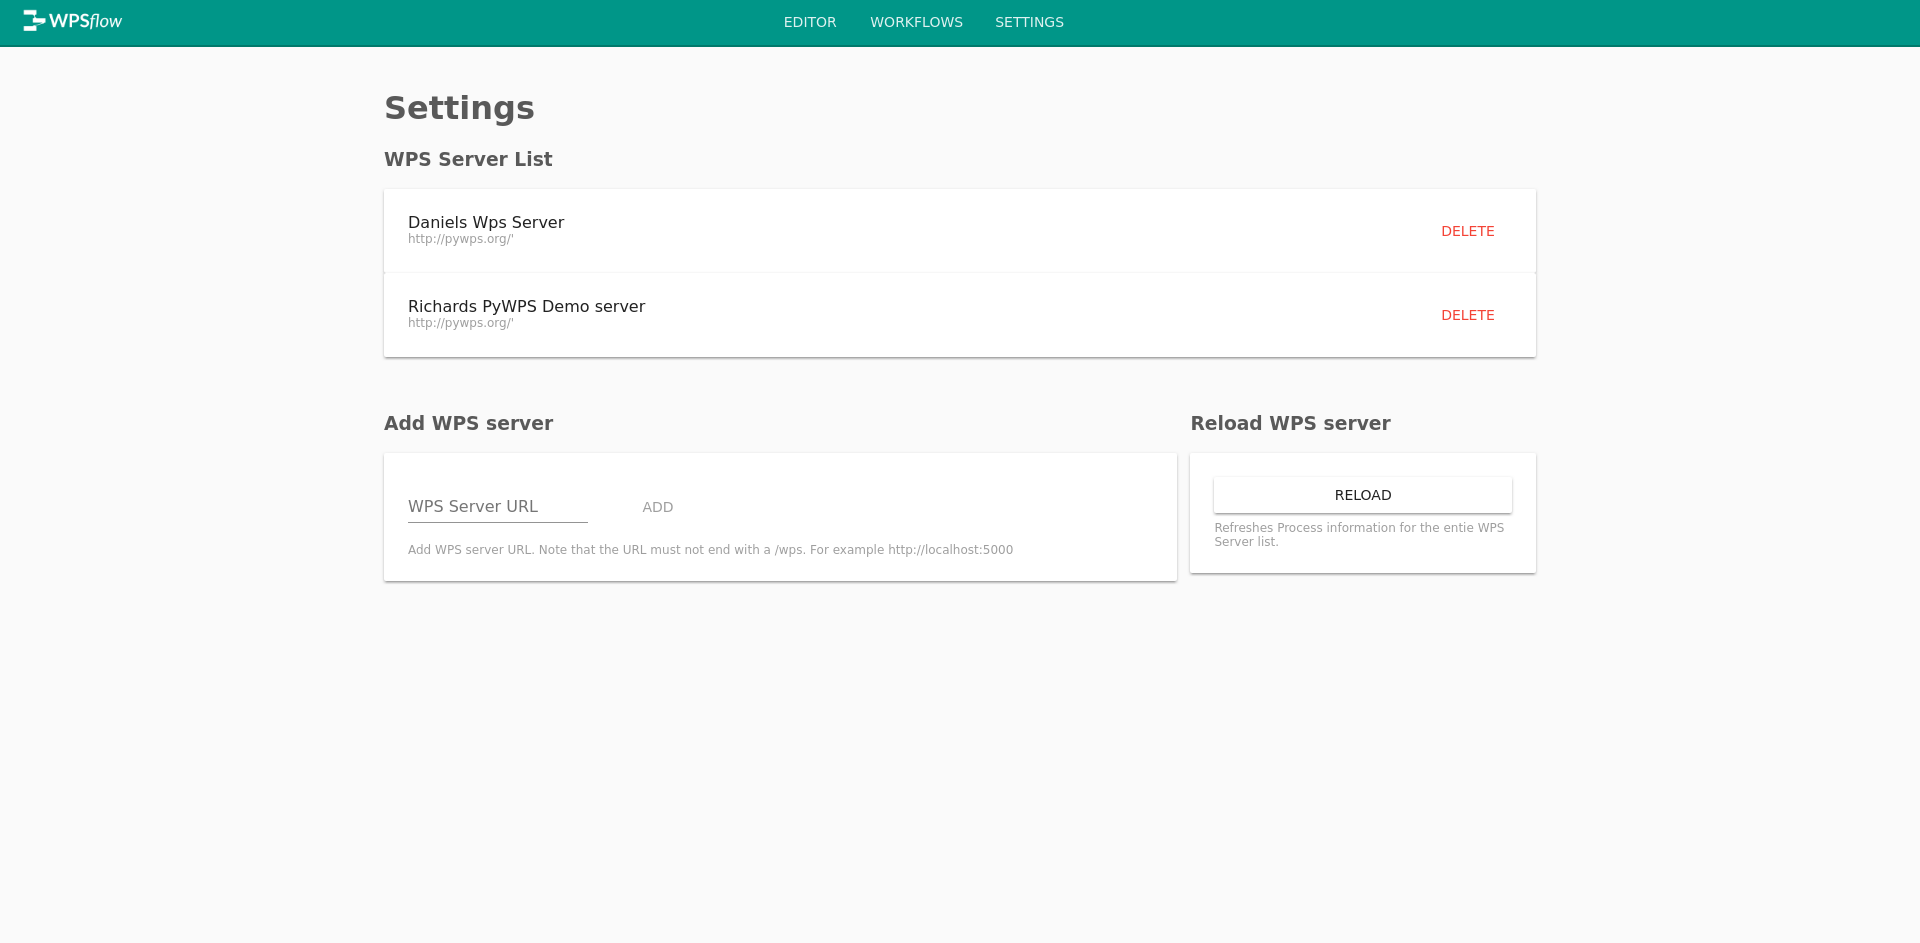
\includegraphics[width=15.5cm]{images/Settings.png}
        \label{settings}
    \end{figure}
    Wenn man ganz oben auf den Einstellungen Knopf drückt, kommt man auf die Einstellungsseite. Hier kann man neue WPS Server hinzufügen, die WPS Tasks anbieten. Diese Tasks, des neuen WPS Servers, werden dann anschließend in der Tasks Übersicht im Editor angezeigt. Man kann auch manuell die Liste an vorhandenen Tasks aktualisieren, indem man auf den reload Knopf drückt. In dem Fall werden alle gespeicherten WPS Server aktualisiert. 